\documentclass[11pt,a4paper]{article}

\usepackage[utf8]{inputenc}
\usepackage[T1]{fontenc}
\usepackage[margin=2.5cm]{geometry}
\usepackage{amsmath, amssymb}
\usepackage{booktabs}
\usepackage{graphicx}
\usepackage{siunitx}
\usepackage{xcolor}
\usepackage{hyperref}
\usepackage{eurosym}
\usepackage{titling}


% TODO marker: remove all \todo{} before submission
\newcommand{\todo}[1]{\textcolor{red}{\textbf{[TODO: #1]}}}

\graphicspath{{figures/}}


\title{\textbf{Euro Coin Image Classification}\\
\large From a Multilayer Perceptron to Cost-Sensitive Transfer Learning}
\author{Claudio Guarrasi\\[1ex]}
\date{\today}

% Subtitle above title (use \pretitle)
\pretitle{%
  \begin{center}
  	\vspace{-3cm} %vertical distance between upper margin and the logo. A negative value means that I am trying to get them closer.
  	\hspace*{0.1cm} %moving it on the right-
    	
\includegraphics[width=0.3\textwidth]{black_unipv_logo_caption_below.png}
	\rule{\textwidth}{0.3pt}
    	\textit{Machine Learning}\\[1ex]
    	\Large  % Switch to large font for the title
}
\posttitle{%
	\end{center} % Close centering.
	}

\preauthor{\begin{center}}
\postauthor{%
	\small{Department of Electrical, Computer and Biomedical Engineering}\\
	\small{University of Pavia}\\[1ex]
	\small{Email: \href{mailto:claudio.guarrasi01@universitadipavia.it}{claudio.guarrasi01@universitadipavia.it}}\\
	%\small{GitHub: \href{https://github.com/PapiDrago/n-body-problem}{\underline{https://github.com/PapiDrago/n-body-problem}}}
	\end{center}}



\begin{document}

\maketitle

\begin{abstract}
This report tackles the classification of euro coin images across the eight
denominations, using a dataset of only 800 training images. Three architectures of
increasing sophistication are developed in sequence, each motivated by the limitations
of the previous one: a multilayer perceptron, a convolutional neural network trained
from scratch, and a pretrained ResNet18 adapted through transfer learning. Test accuracy
rises from approximately 70\% for the MLP to 79\% for the CNN and 96\% for the
fine-tuned ResNet18, confirming that on small datasets reusing features learned on a
large dataset clearly outperforms training from scratch. A second objective, minimizing
the ``value of misclassification'' (the mean absolute difference between predicted and
true face value), is addressed with a cost-sensitive decision rule that requires no
retraining. This rule leaves the confident ResNet unchanged but, on the less certain
MLP, lowers the average misclassification cost by steering both its corrections and its
residual errors toward coins of nearer value.
\end{abstract}

\tableofcontents

\section{Introduction}
\label{sec:intro}

This report addresses the task of classifying images of euro coins into their eight
classes (1c, 2c, 5c, 10c, 20c, 50c, 1\officialeuro{}, 2\officialeuro{}).
Coin classification is not an easy task because there is a large number of different
coin series in circulation, issued in different European Union countries. Each coin
series can have numerous variations, such as different legends, mint marks, symbols, and
designs, making classification a challenge even for human experts. Each member of the
European monetary union has its own version of the coins, with one side representing
European unity and the other side featuring a national design. For a more exhaustive
discussion of the difficulties of coin classification, see Cirillo et al.~\cite{cirillo2024}.
 
Two objectives are pursued. The first is the standard one: minimizing the classification
error. The second is the design of an additional model that minimizes the
``value of misclassification'', defined as the mean absolute difference between the
predicted and the true face value of the coin (e.g., a 50-cent coin misclassified as a
20-cent coin costs 30 points).
 
The methodology follows a progression of three architectures of increasing
sophistication --- a multilayer perceptron (MLP), a convolutional neural network (CNN)
trained from scratch, and a pretrained ResNet18 adapted via transfer learning --- where
each step is motivated by the empirically observed limitations of the previous one. The
cost-sensitive objective is then addressed on top of the best model through a decision
rule driven by the specification of costs for correct and incorrect predictions, without
any retraining.

\section{Dataset and preprocessing}

\subsection{Dataset}

The dataset is organized in an \texttt{ImageFolder} structure, split into a training set folder and a test set folder. In each of those folder we have one directory per class. The images are RGB PNG files of size 64 x 64 pixels.
In the training set folder there are 100 images per class, whereas in the test set folder the images per class are 20 giving a grand-total of 800 images in the training set and 160 images in the test set, making this a small-data image classification problem.

Fortunately the classes are all equally represented, meaning that all the classes will have the same effect on the overall loss. In other terms, the model can “focus its attention” on all classes.

In addition the images have been taken with variable noise, sharpness, lighting conditions, and
backgrounds. They can be face up or down, and can be rotated in any direction. With the hope to convey enough variability in the dataset. Examples of train image samples can be seen in Figure~\ref{fig:samples}).

 \begin{figure}[ht]
   \centering
   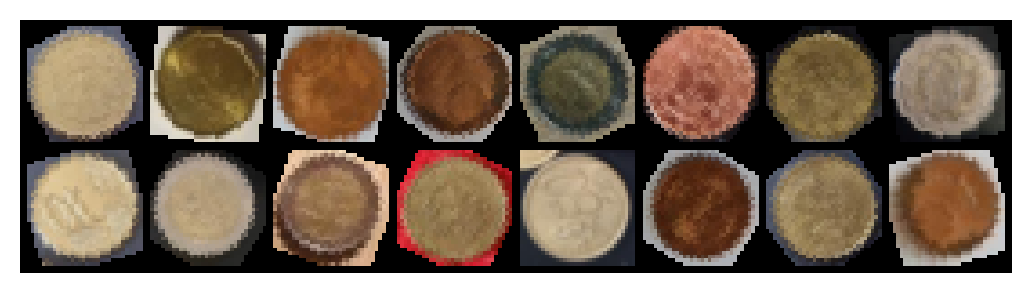
\includegraphics[width=0.9\textwidth]{train_samples.png}
   \caption{Sample images from the training set.}
   \label{fig:samples}
 \end{figure}

\subsection{Transforms and data augmentation}
All the images in the dataset were already cropped allowing to have just one coin per image.

The following preprocessing and data augmentation techniques were applied on the images in order to allow them to be suitable for deep learning models and to improve their training phase.

All images are resized, converted to tensors, and normalized with the ImageNet per-channel statistics in order to move the provided dataset distribution towards the same one the ResNet18 was trained ob. The input resolution depends on the model: 32×32 for the MLP and CNN, chosen mainly to lighten the computations of the MLP given its large number of parameters, and 224×224 for ResNet18, matching the resolution at which it was pretrained.
Data augmentation is applied to the training set only: random horizontal flips and
random rotations. Augmentation artificially increases the effective size of a small
dataset and is applied at runtime, so the model never sees exactly the same input twice
across epochs. The test set receives only the deterministic preprocessing (resize,
tensor conversion, normalization), so that the evaluation reflects the real data
distribution.

Rotation is a particularly natural augmentation for coins, which have no canonical
orientation in real photographs. However, the appropriate rotation amplitude turned out
to depend on the model: aggressive $180°$ rotations helped the networks trained
from scratch, but degraded the pretrained ResNet, whose ImageNet features are
orientation-dependent. This is discussed in Section~\ref{sec:resnet}.

\subsection{Data loading}

Data is loaded with PyTorch \texttt{DataLoader}s using a batch size of 16 with shuffling
on the training set. With only 800 training images, a relatively small batch size yields
more parameter updates per epoch. In addition because the gradient is computed on a few samples, this gives a poor estimate of the true gradient: a noisier estimate tends to help the model to escape sharp minima (narrow valley in the loss function that tends to overfit the training data) and land on flat minima.
\section{Model progression}

Three models were developed in sequence. Each subsection describes the architecture,
the training configuration, the diagnostic process, and the results; the comparison is
summarized in Table~\ref{tab:comparison}.

\subsection{Multilayer perceptron}
For a detailed treatment of multilayer perceptrons (MLP), see~\cite{pml1Book}.

With only 800 images in the training set a huge network (in terms of depth) would overfit immediately.
However only a single hidden layer would give the model too little capacity to learn meaningful features combinations from $32 \times 32 \times 3$ input values because the pattern detection capability is limited to just one level of abstraction: the model is forced to go directly to class predictions from raw pixels.

Whereas three or more layers would have too many parameters relative to the data, leading to overfitting.
Two layers seems the right balance. Here is the 2-hidden layer MLP structure:

The architecture is a funnel of two hidden layers
($3072 \to 512 \to 256 \to 8$) in order to go from low level features to higher level features with the purpose of classifying correctly the coins. In each hidden block the linear layer is followed by batch normalization, ReLU activation,
and dropout  The output layer produces raw logits, since the cross-entropy
loss applies the softmax internally. Given the very high ratio of parameters to
training samples ($\approx$1.7M parameters for 800 images), the following normalization/regularization mechanisms were employed: 
\begin{itemize}
  \item \textbf{Dropout} randomly deactivates a fraction $p$ of neurons at each
  training step. This prevents the network from relying too heavily on any single
  neuron and forces it to learn redundant representations distributed across many
  units, which improves generalization. In this experiment $p$ was set to $0.3$
  \item \textbf{Batch normalization} standardizes the output of each linear layer to
  approximately zero mean and unit variance before the activation. This counteracts the
  shifting of internal activation distributions during training, stabilizing and
  accelerating optimization; it also has a mild regularizing effect.
 \item \textbf{L2 weight decay} adds a penalty proportional to the squared magnitude of
the weights to the loss, discouraging large weights and thus favoring simpler,
smoer functions that are less prone to overfitting. In this experiment the 
L2 weight-decay coefficient $\lambda$ was set to $10^{-4}$.
\end{itemize}
\paragraph{Training diagnostics.}
The initial configuration (Adam optimizer, learning rate $10^{-3}$) produced an oscillating training loss produced an oscillating training
loss and an accuracy plateau around 63\%, a typical symptom of a learning rate large
enough to repeatedly overshoot the minimum. Lowering the learning rate to $10^{-4}$ and
doubling the number of epochs raised the accuracy to approximately 70\%, with reduced
but still present oscillation. Adding a \texttt{ReduceLROnPlateau} scheduler did not
yield further improvement: the loss kept oscillating and the test accuracy did not
increase. This indicated that the bottleneck was no longer the optimization but the
architecture itself --- an MLP discards all spatial structure, treating each pixel
independently, and has neither locality nor translation invariance, a limitation made harder to overcome by the small training set.

\begin{figure}[ht]
   \centering
   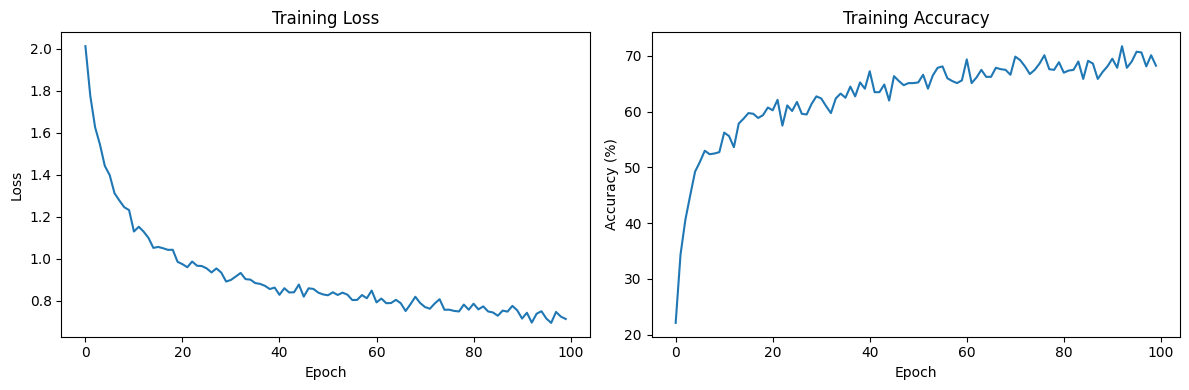
\includegraphics[width=0.9\textwidth]{mlp_train_measures.png}
   \caption{Training loss and accuracy curves, showing clear oscillations.}
   \label{fig:mlp_train_measures}
 \end{figure}

\subsection{Convolutional neural network (from scratch)}
For a detailed treatment of convolutional neural networks (CNN), see~\cite{pml1Book}.
The CNN consists of three convolutional blocks, each following the pattern
Conv($3 \times 3$, padding 1) $\to$ BatchNorm $\to$ ReLU $\to$ MaxPool($2 \times 2$),
with channel widths doubling across blocks ($32 \to 64 \to 128$) as the spatial
resolution halves ($32 \to 16 \to 8 \to 4$). A compact classifier head
($2048 \to 256 \to 8$ with dropout) completes the network. Despite being a more
expressive architecture, the CNN has roughly five times fewer parameters than the MLP
($\approx$345K vs $\approx$1.7M), thanks to weight sharing in the convolutional layers.

The number of output channels is doubled at each block in order to compensate for the
spatial-dimension shrinkage caused by pooling. The $3 \times 3$ convolutions use
padding~1 to preserve the spatial size (same-size convolution), so that the role of
reducing the resolution is delegated solely to the pooling layers.

Trained with the same loop and hyperparameters as the MLP, the CNN reached 86\% training
accuracy and 79\% test accuracy. The $\approx$7-point gap indicates mild, acceptable
overfitting for a network trained from scratch on 800 images. The training loss still
did not converge smoothly, consistent with the small number of batches per epoch (50)
and the resulting gradient noise.

The confusion matrix (Figure~\ref{fig:cnn_matrix}) reflects the model's accuracy:
predictions concentrate on the diagonal. The few remaining errors occur predominantly
between visually similar classes, such as the small copper coins (1c, 2c, 5c).

\begin{figure}[ht]
   \centering
   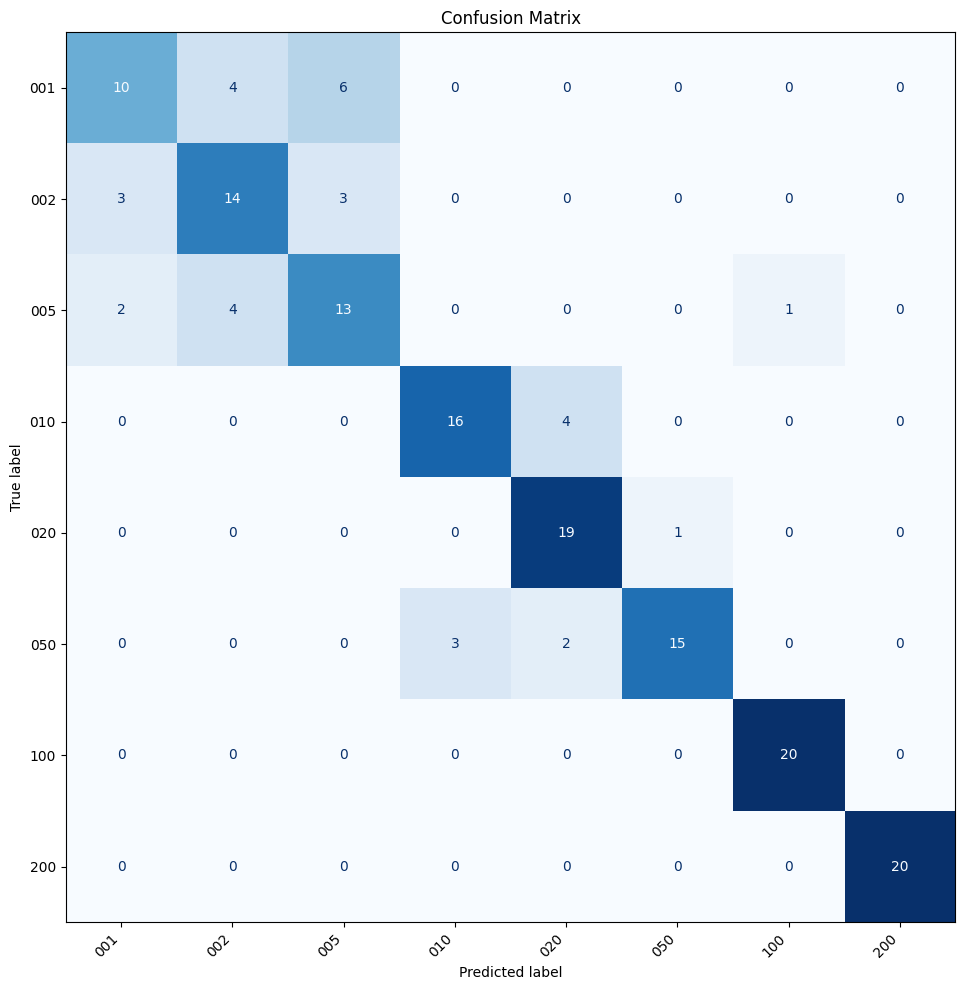
\includegraphics[width=0.7\textwidth]{cnn_confusion_matrix.png}
   \caption{Confusion matrix of the from-scratch CNN on the test set. Rows are true
   classes, columns are predicted classes.}
   \label{fig:cnn_matrix}
\end{figure} 
\subsection{Transfer learning with ResNet18}
\label{sec:resnet}

For a detailed introduction to ResNets, see~\cite{he2016deep}.

To overcome the problems of having a small training set preventing a CNN and in general a model from learning meaningful representations from scratch with limited data, we can leverage pre-trained networks. It is a good idea because low and mid level features such as edges, textures and shapes are universal across image domains, making features learned on huge datasets, like ImageNet dataset, transferable to new tasks.

A pretrained ResNet18 was chosen as the smallest member of the ResNet family. Its residual
(skip) connections allow gradients to flow directly across layers, mitigating the
vanishing-gradient problem and enabling stable training of deep networks. Among the
available depths (18, 34, 50, \dots), the 18-layer variant is the most appropriate here:
with only 800 training images, a larger backbone would offer more capacity than the data
can support and would increase the risk of overfitting during fine-tuning, while also
being slower to train. ResNet18 therefore provides a strong pretrained feature extractor
at a model size proportionate to the dataset.

Adapting a pretrained network to a new task is known as \emph{transfer learning}, and
the process of unfreezing some or all of its weights and continuing training on the
target data is called \emph{fine-tuning}. Training proceeded in two phases: the new
classification head is first trained alone so that its initially random weights settle
to reasonable values, before the whole network is fine-tuned. This ordering avoids large,
poorly-directed gradients from an untrained head propagating back and disturbing the
valuable pretrained features.

\begin{description}
  \item[Phase 1 (frozen backbone).] All pretrained layers were frozen and only the new
  final layer ($\approx$4K trainable parameters) was trained with Adam
  (lr $10^{-3}$, weight decay $10^{-4}$).
  \item[Phase 2 (fine-tuning).] All layers were then unfrozen and trained with a much
  lower learning rate ($10^{-4}$), so that the pretrained convolutional weights were
  gently adapted to coin-specific features rather than overwritten.
\end{description}

\paragraph{Training diagnostics.}
Phase 1 initially underperformed ($\approx$60--66\% accuracy). Two causes were
identified. First, an excessive learning rate ($10^{-1}$) in an early run. Second, and
more interesting, the \ang{180} random rotation, which had helped the models
trained from scratch, degraded the pretrained features, which are orientation-dependent
because ImageNet objects have a canonical orientation. Reducing the rotation to
\ang{15} was empirically the best setting (Table~\ref{tab:rotation}).
 
 
\begin{table}[ht]
  \centering
  \begin{tabular}{lcc}
    \toprule
    Rotation amplitude & Train accuracy & Test accuracy \\
    \midrule
    \ang{\pm15} & 82\% & 77.5\% \\
    \ang{\pm30} & 75\% & 74\% \\
    \bottomrule
  \end{tabular}
  \caption{Effect of rotation augmentation amplitude on Phase 1 of transfer learning.}
  \label{tab:rotation}
\end{table}
 
 \begin{figure}[ht]
   \centering
   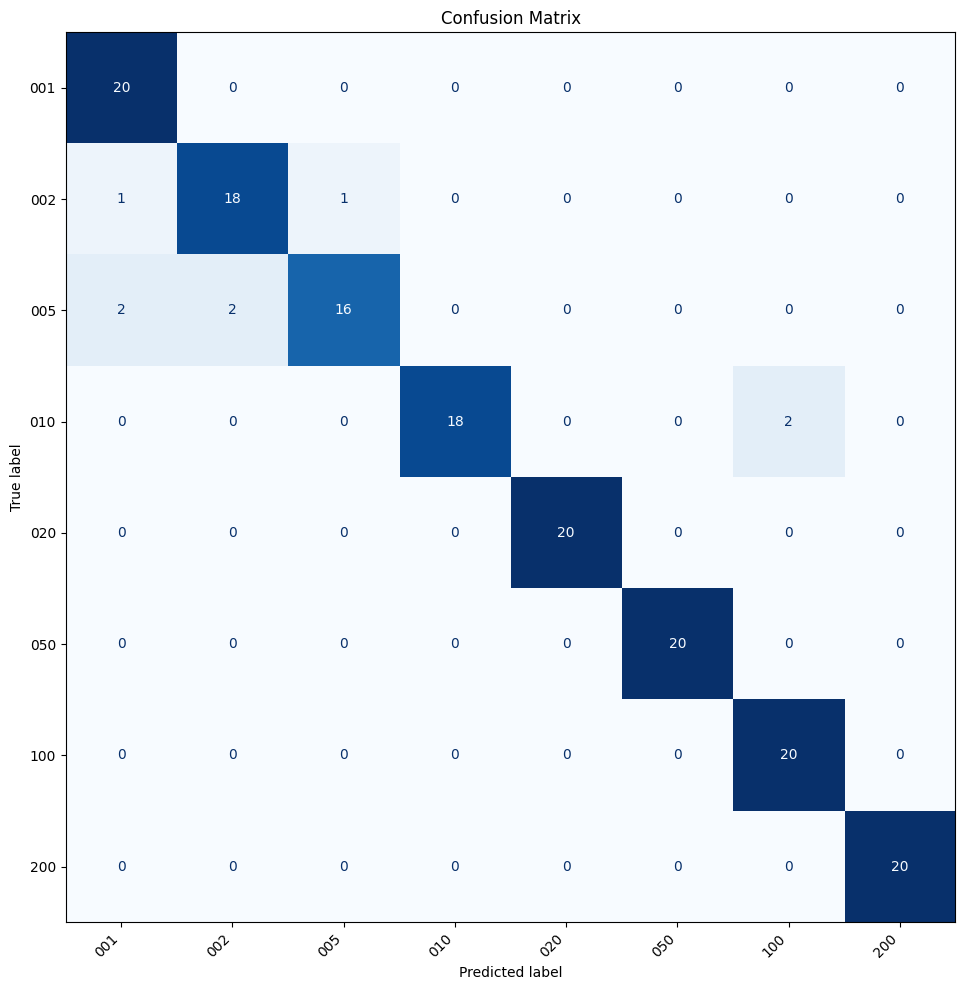
\includegraphics[width=0.7\textwidth]{resnet_matrix.png}
   \caption{Confusion matrix of the ResNet18 on the test set. Rows are true~classes, columns are predicted~classes.}
   \label{fig:resnet_matrix}
\end{figure}

With this configuration, Phase 1 converged to approximately 77\% train / 75\% test
accuracy. Fine-tuning in Phase 2 produced a dramatic improvement to 99\% training and
96\% test accuracy, with training converging by approximately epoch 40 (motivating
early stopping, see Section~\ref{sec:limitations}). The 3-point train/test gap
indicates minimal overfitting.

\subsection{Model comparison}

\begin{table}[ht]
  \centering
  \begin{tabular}{lccc}
    \toprule
    Model & Total params & Trainable params & Test accuracy \\
    \midrule
    MLP & $\approx$1.71M & $\approx$1.71M & $\approx$70\% \\
    CNN (from scratch) & $\approx$345K & $\approx$345K & 79.4\% \\
    ResNet18 -- Phase 1 (frozen) & $\approx$11.2M & $\approx$4.1K & 75\% \\
    ResNet18 -- Phase 2 (fine-tuned) & $\approx$11.2M & $\approx$11.2M & 96\%  \\
    \bottomrule
  \end{tabular}
  \caption{Summary of the model progression. Note the contrast between total and
  trainable parameters in Phase 1.}
  \label{tab:comparison}
\end{table}

The progression illustrates two classical lessons of small-data image classification:
convolutional inductive biases beat fully connected architectures at a fraction of the
parameter cost, and reusing representations learned on a large dataset dominates
training from scratch.

\section{Cost-sensitive classification}

\subsection{Motivation and theory}

Classification accuracy treats all errors as equally severe, but in this application
misclassifying a 2\officialeuro{} coin as 1c is far more damaging than confusing 10c with 20c.
The requested metric is the mean absolute difference between predicted and true face
value. This is a cost-sensitive learning problem~\cite{elkan2001foundations}, with cost matrix
\begin{equation}
  C(i, j) = \lvert v_i - v_j \rvert,
\end{equation}
where $v \in \{1, 2, 5, 10, 20, 50, 100, 200\}$ (cents) indexes the eight
denominations.

The Bayes-optimal decision rule under a cost matrix replaces the argmax over class
posteriors with the minimization of the conditional risk:
\begin{equation}
  R(i \mid x) = \sum_{j=0}^{7} P(y = j \mid x)\, C(i, j),
  \qquad
  \hat{y} = \arg\min_i\, R(i \mid x).
  \label{eq:risk}
\end{equation}

Crucially, the network does not need to be retrained: minimizing the standard
cross-entropy already drives the softmax output toward an estimate of the posterior
$P(y \mid x)$, which is exactly the quantity Equation~\eqref{eq:risk} requires. The
cost-sensitive model is therefore the same trained network equipped with a different
decision rule at inference time. This has the practical advantage that a single trained
model supports any cost matrix, and the two requested models (accuracy-optimal and
cost-optimal) share all of their weights.
\subsection{Results}
 
With the fine-tuned ResNet18, the risk-minimizing rule made the same predictions as the
standard argmax rule, leaving the misclassification cost unchanged. This happens because
the cost-sensitive rule can only improve on argmax when the model is uncertain: it then
hedges toward a coin whose value is close to the likely alternatives, limiting the damage
of a possible mistake. Since the ResNet is highly accurate and confident, it leaves almost
no uncertainty to exploit, and the two rules coincide.
 
To appreciate the mechanism, we therefore evaluate it on the weaker and less confident MLP
(Table~\ref{tab:cost}), where the cost-sensitive rule does reduce the average
misclassification cost.
 
\begin{table}[ht]
  \centering
  \begin{tabular}{lc}
    \toprule
    Decision rule (MLP) & Mean misclassification cost (cents) \\
    \midrule
    argmax (standard) & 4.47 \\
    risk-minimizing (cost-sensitive) & 3.48 \\
    \bottomrule
  \end{tabular}
  \caption{Mean absolute face-value error of the two decision rules, evaluated on the MLP.}
  \label{tab:cost}
\end{table}
 
The improvement comes from the way the rule handles uncertain cases: when the model is
unsure, it favors the coin whose value is closest to the likely alternatives. Sometimes
this recovers the correct class outright (for instance a 20c coin that argmax had
confused with 50c); in other cases the prediction stays wrong but lands on a coin of
nearer value, so the error becomes cheaper (for instance a 1c coin confused with 5c
rather than with 50c). Either way, the rule lowers the average cost not by guaranteeing
more correct answers, but by steering both its corrections and its residual mistakes
toward coins of similar value.
\section{Conclusions}

This work classified euro coin images under two objectives. For classification error, a
progression MLP $\to$ CNN $\to$ fine-tuned ResNet18 raised test accuracy from
$\approx$70\% to 96\%, confirming that on small datasets transfer learning is
decisively superior to training from scratch. For the value of misclassification, a
Bayes-optimal cost-sensitive decision rule applied to the same trained network reduced
the mean absolute face-value error, essentially for free, by trading a small number of
cheap errors for the elimination of rare but expensive ones.

\section{Limitations and future work}
\label{sec:limitations}

\begin{itemize}
  \item \textbf{Validation methodology.} Hyperparameters were tuned by observing test
  performance, since no validation split was used. A rigorous protocol would hold out a
  validation set (or use cross-validation) and touch the test set only once.
  \item \textbf{Early stopping.} Fine-tuning converged by epoch $\approx$40 of 50; an
  early-stopping criterion with best-model checkpointing would make training more
  efficient and guard against late-stage overfitting.
  \item \textbf{Dataset size and variability.} With 800 training images, results carry
  non-negligible run-to-run variance; averaging over multiple seeds would strengthen
  the conclusions.
\end{itemize}

\section*{Declaration of AI tool usage}
\addcontentsline{toc}{section}{Declaration of AI tool usage}

In accordance with the assignment guidelines, I declare that AI tools (Claude, Anthropic)
were used for the following tasks:
\begin{itemize}
  \item Debugging code issues, such as loading the dataset from Google Drive and
  diagnosing the cause of training instabilities (e.g.\ the oscillating loss and the
  Phase~1 underperformance of the transfer-learning model).
  \item Discussing and clarifying machine learning concepts, including the choice of
  batch size, regularization mechanisms, data augmentation, and the theory of
  cost-sensitive classification.
  \item Assisting with the drafting, structuring, and wording of this report, including
  the generation of the \LaTeX{} template.
\end{itemize}
All design decisions, experiments, results, and their interpretation are my own, and the
content has been reviewed and validated by me.

\vspace{1em}

\noindent ``I affirm that this report is the result of my own work and that I did not
share any part of it with anyone else except the teacher.''

\begin{thebibliography}{9}
 
\bibitem{cirillo2024}
Cirillo, S., Solimando, G. \& Virgili, L.
\newblock A deep learning approach to classify country and value of modern coins.
\newblock \emph{Neural Computing and Applications} \textbf{36}, 11759--11775 (2024).
\newblock \url{https://doi.org/10.1007/s00521-023-09355-6}
 
 \bibitem{pml1Book}
Murphy, K. P.
\newblock \emph{Probabilistic Machine Learning: An Introduction}.
\newblock MIT Press (2022).
\newblock \url{http://probml.github.io/book1}

\bibitem{he2016deep}
He, K., Zhang, X., Ren, S. \& Sun, J.
\newblock Deep residual learning for image recognition.
\newblock In \emph{Proceedings of the IEEE Conference on Computer Vision and Pattern
Recognition (CVPR)}, 770--778 (2016).

\bibitem{elkan2001foundations}
Elkan, C.
\newblock The foundations of cost-sensitive learning.
\newblock In \emph{Proceedings of the 17th International Joint Conference on Artificial
Intelligence (IJCAI)}, vol.~17, no.~1, 973--978 (2001).
 
\end{thebibliography}

\end{document}
